% !TeX spellcheck = ru_RU
% !TEX root=../main.tex

\begin{lecture}[Растворы и взаимная растворяемость]
	Вследствие шубы имеем поправку на потенциал: $ \phi (r) = \dfrac{e^2}{\eps r} e^{-\kappa r} $.
	Характерный радиус $ \lambda  = \sqrt{\dfrac{\eps k T}{8 \pi e^2 n}}~\Rightarrow~ U = -\dfrac{e^2 \kappa}{\eps}$.
	\begin{lecSection}[Ионные жидкости]
		При $ T \rightarrow 800^\circ C $ расплав, $ 10 - 25 \% $, % TODO: ЧТО ТАМ НАПИСАНО В КОНСПЕКТЕ??
		
		То есть, \underline{в структуре расплава появляются полости}.
		
		Есть вещества, являющиеся ионными жидкостями при комнатной температуре, например, RTIL.
		\begin{figure}[h]
			\centering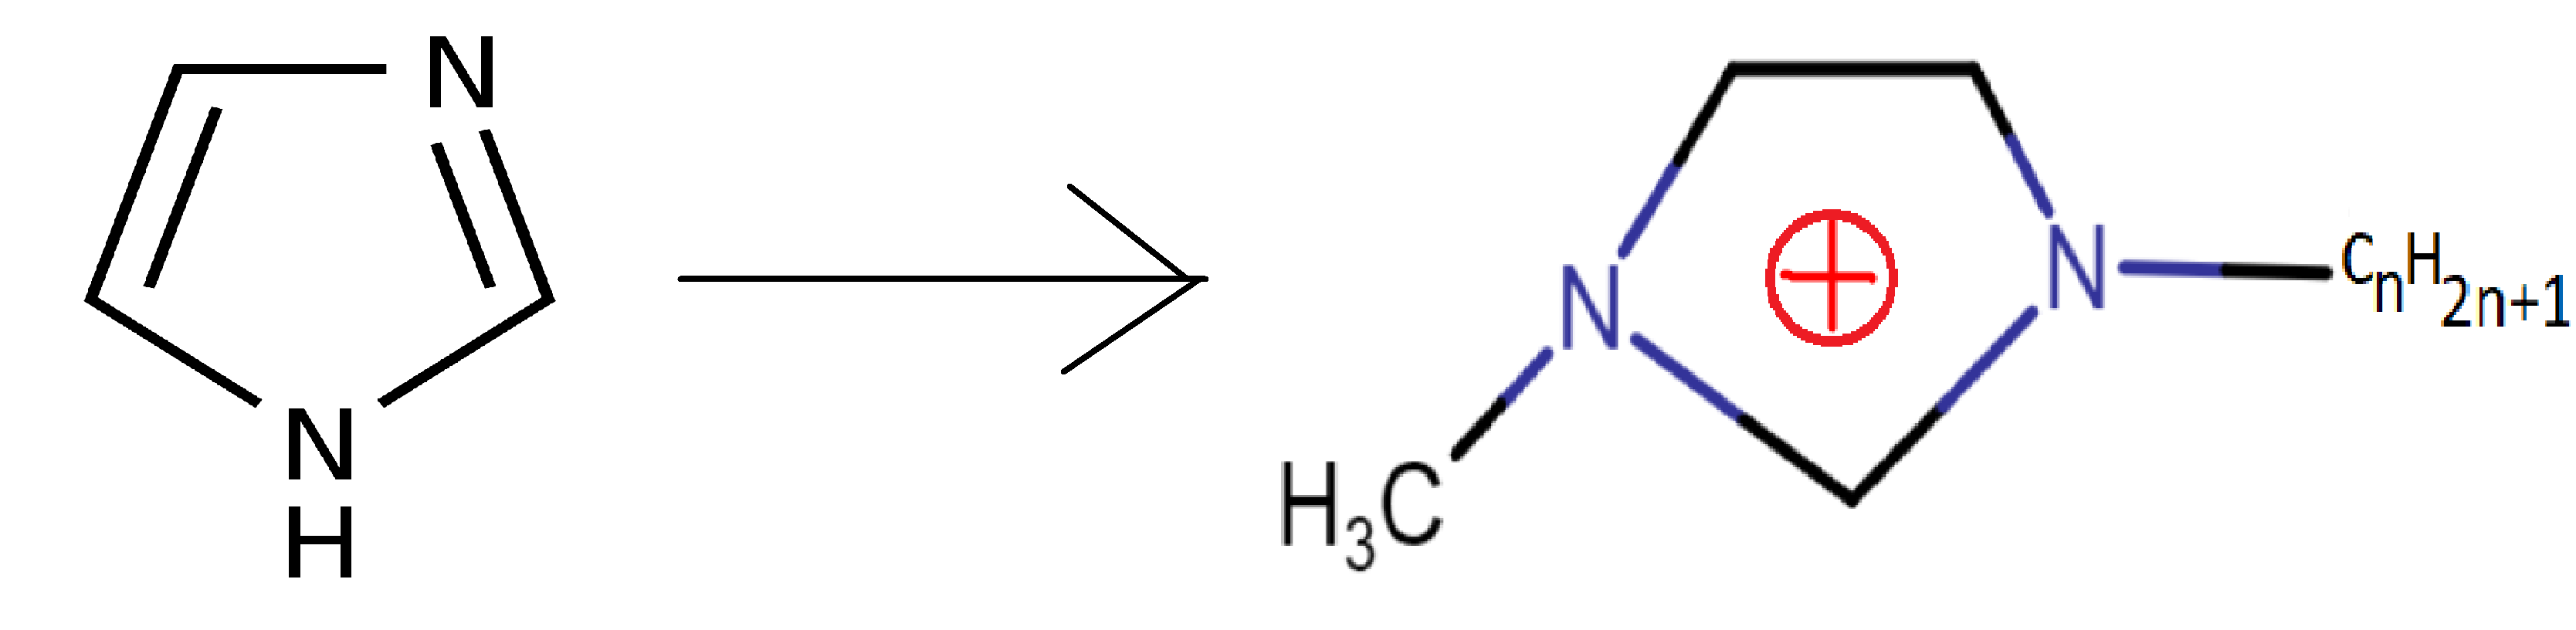
\includegraphics[width=0.8\linewidth]{lecture_11/imidazole}
			\caption{Превращение имидазола}
			\label{fig:11:imid_transform}
		\end{figure}
		
		\begin{figure}[h]
			\begin{minipage}{0.48\linewidth}
				\centering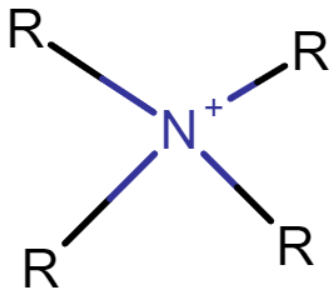
\includegraphics[width=0.7\linewidth]{lecture_11/alkil_ammon}
				\caption{Алкиламмоний}
				\label{fig:11:alkilammon}
			\end{minipage}
			\begin{minipage}{0.48\linewidth}
				\centering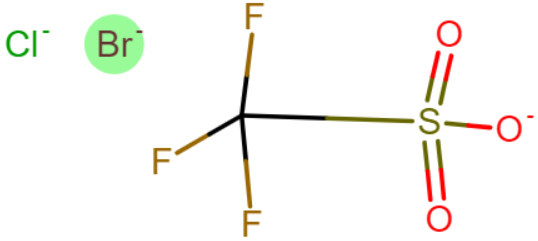
\includegraphics[width=\linewidth]{lecture_11/pic3}
				\caption{3-флюрометан сульфонат}
				\label{fig:11:metan_sulfonat}
			\end{minipage}
		\end{figure}
	
		ИЖ -- нелетучие, негорючие, наноразмерные неоднородности, $ \eps \sim 10 $, высокая вязкость.
		
		Можно смешивать с органическими растворами, что снижает вязкость.
		
		\underline{Использование}:
		\begin{itemize}
			\item Медицина (комплекс)
			\item В качестве растворителей
			\item В ядерных технология (жидкая экстракция)
		\end{itemize}
	
		\textit{Пример}: несмешиваемые $ A $ и $ B $. При этом $ C $ растворяется в обоих. Как распределится $ C $ между $ A $ и $ B $?
		
		\begin{gather*}
			d G = \sum\limits_i \mu_i dN_i = 0 ~\text{-- общая формула} \\
			= \mu_A dn_A - \mu_B dn_A = 0
		\end{gather*}
		где $ \mu_A $ -- потенциал в $ A $, $ \mu_A = \mu_B $ в равновесии.
		\begin{gather*}
		\mu_A^0 + RT \ln C_A = \mu_B^0 + RT \ln C_B \\
		\dfrac{C_A}{C_B} = \exp \left( \dfrac{\mu_B^0 - \mu_A^0}{RT}\right) = D~\text{-- коэффициент распределения}
		\end{gather*}
	\end{lecSection}
\end{lecture}